This section of the assignment implements a Linux Kernel Module in order to read
and write the RTC time. The ``rtc-ds1307.ko'' LKM is compatible with the DS3231,
and will be used for this section. The Linux ``modprobe'' program is used to add
the LKM to the kernel. The ds1307 device is then instantiated by writing its
address to the i2c-1 directories ``new\_device'' file. This process can be seen
in Figure \ref{fig:images-lkm1}.

\begin{figure}[H]
	\centering
	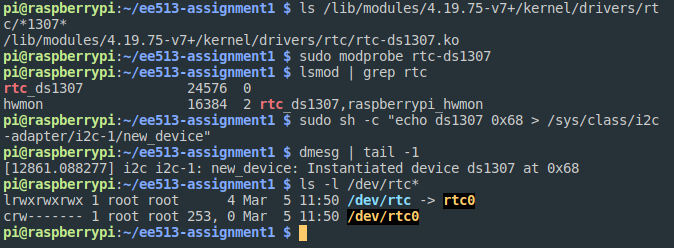
\includegraphics[width=0.8\textwidth]{images/lkm1}
	\caption{Adding the DS1307 LKM to the Kernel}
	\label{fig:images-lkm1}
\end{figure}

Executing the ``i2cdetect'' command shows a value of ``UU'' at the RTC's
address, showing the device is in use by an LKM.

\begin{figure}[H]
	\centering
	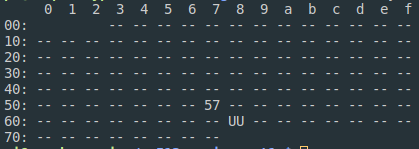
\includegraphics[width=0.8\textwidth]{images/lkm2}
	\caption{i2cdetect Output}
	\label{fig:images-lkm2}
\end{figure}

By navigating to the devices ``sysfs'' entry, the ``cat'' command can be used to
output the current RTC time to the user.

\begin{figure}[H]
	\centering
	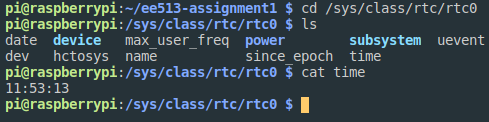
\includegraphics[width=0.8\textwidth]{images/lkm3}
	\caption{RTC output via the ``cat'' command}
	\label{fig:images-lkm3}
\end{figure}

The ``hwclock'' utility can also be used to read or write to the RTC, with the
``set'' option allowing for the system time to be set from the RTC.

\begin{figure}[H]
	\centering
	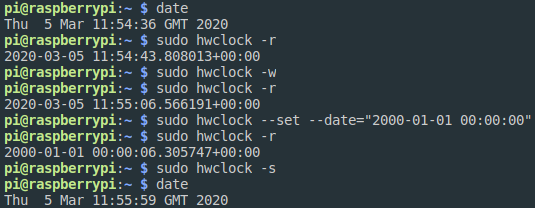
\includegraphics[width=0.8\textwidth]{images/lkm4}
	\caption{``hwclock'' utility usage}
	\label{fig:images-lkm4}
\end{figure}

To automatically set the time via the RTC at boot time, a systemd service can be
added to the ``system'' directory. The contents of this service file can be seen
in Figure \ref{fig:images-lkm5}.

\begin{figure}[H]
	\centering
	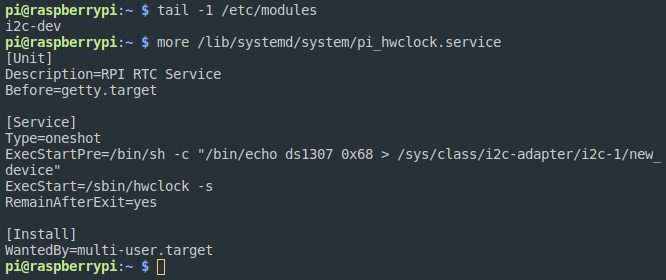
\includegraphics[width=0.8\textwidth]{images/lkm5}
	\caption{System service integration}
	\label{fig:images-lkm5}
\end{figure}

In order to start this service, the ``systemctl'' command can be run. The NTP
service must also be disabled, however, as shown in Figure \ref{fig:images-lkm6}, the
``ntp'' service is not available. This is because it is no longer included in
the Raspbian Stretch images.

\begin{figure}[H]
	\centering
	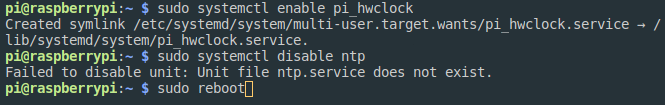
\includegraphics[width=0.8\textwidth]{images/lkm6}
	\caption{Enabling the system service}
	\label{fig:images-lkm6}
\end{figure}

Once the system has been rebooted, the status of this system service can be
checked. Figure \ref{fig:images-lkm7} shows that the service is active after a
reboot.

\begin{figure}[H]
	\centering
	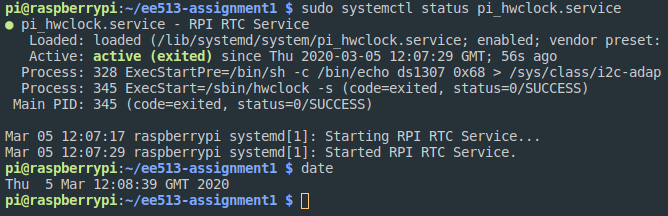
\includegraphics[width=0.8\textwidth]{images/lkm7}
	\caption{System service status}
	\label{fig:images-lkm7}
\end{figure}

Finally, in order to remove the LKM and undo the creation of the system service,
the service must be disabled, with the ntp service re-enabled. As mentioned,
this service no longer exists within the Raspbian Stretch images. The LKM can
then be removed by passing the RTC address (0x68) to the ``delete\_device'' file
of the ``i2c-1'' directory. This can be verified using the ``i2cdetect''
command, which shows the address 0x68 for the RTC, indicating it is no longer in
use by the LKM.

\begin{figure}[H]
	\centering
	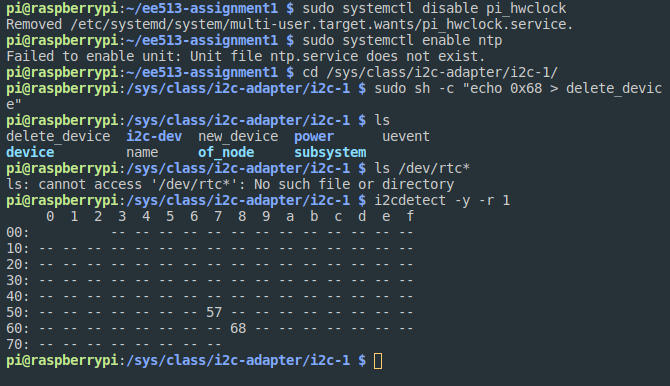
\includegraphics[width=0.8\textwidth]{images/lkm8}
	\caption{Removing the LKM and freeing the RTC}
	\label{fig:images-lkm8}
\end{figure}
